% Editable reconstruction; interpretation recorded in root.json.
% Shared standalone design for the editable figure reconstructions.
\documentclass[tikz,border=5pt,10pt]{standalone}
\usepackage[T1]{fontenc}
\usepackage[utf8]{inputenc}
\usepackage{newpxtext,newpxmath}
\usepackage[scaled=.94]{sourcesanspro}
\usepackage{pgfplots}
\pgfplotsset{compat=1.18}
\usetikzlibrary{arrows.meta,calc,positioning,decorations.pathreplacing,
  decorations.markings,patterns,matrix,shapes.geometric,fit,backgrounds,
  intersections,angles,quotes}
\definecolor{ink}{HTML}{203746}
\definecolor{accent}{HTML}{146C78}
\definecolor{muted}{HTML}{667780}
\definecolor{signalred}{HTML}{B94B44}
\color{ink}
\tikzset{>=Latex,line width=.8pt,
  every node/.style={font=\small},
  axis/.style={->,draw=muted,line width=.5pt},
  guide/.style={draw=muted,dashed,line width=.45pt},
  curve/.style={draw=accent,line width=1pt},
  marker/.style={circle,fill=accent,inner sep=1.5pt},
  labelbox/.style={fill=white,inner sep=2pt}}

\begin{document}

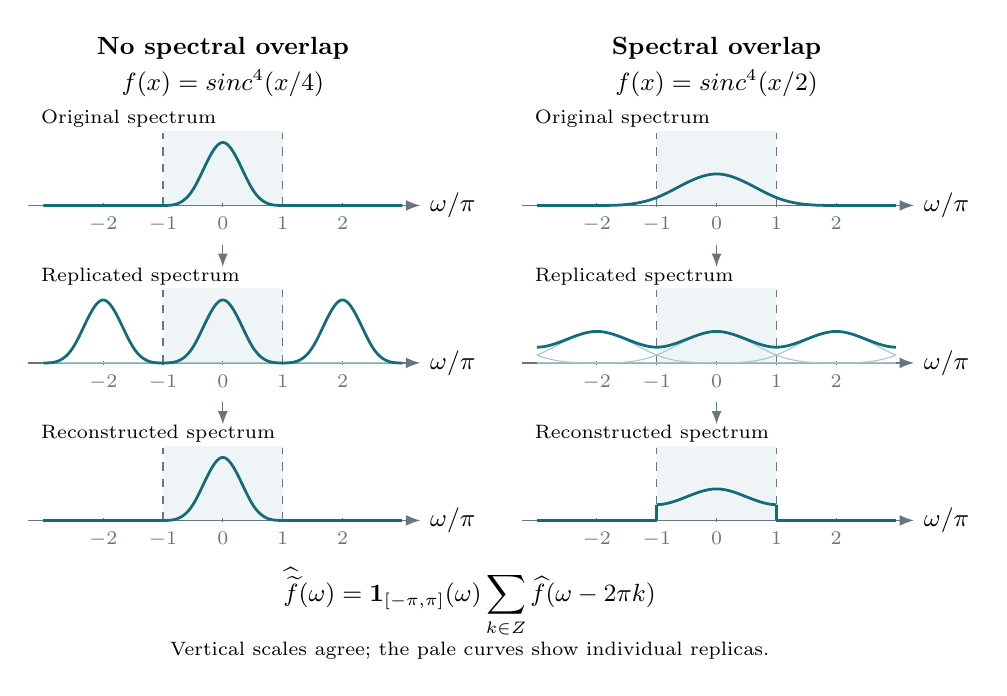
\begin{tikzpicture}[x=.76cm,y=1cm]
\pgfmathdeclarefunction{bs}{1}{\pgfmathparse{(max(0,2-abs(#1))^3-4*max(0,1-abs(#1))^3)/6}}
\foreach \offset/\aa/\heading in {0/4/No spectral overlap,8.25/2/Spectral overlap}{
\begin{scope}[shift={(\offset,0)}]
\node[font=\small\bfseries] at (0,2.0) {\heading};
\node at (0,1.55) {$f(x)=\operatorname{sinc}^{4}(x/\aa)$};
\foreach \yy/\stage in {0/Original spectrum,-2/Replicated spectrum,-4/Reconstructed spectrum}{
\begin{scope}[shift={(0,\yy)}]
\fill[accent!7] (-1,0) rectangle (1,.95);
\draw[axis] (-3.25,0)--(3.3,0) node[right] {$\omega/\pi$};
\draw[guide] (-1,0)--(-1,.92) (1,0)--(1,.92);
\foreach \q in {-2,-1,0,1,2}{\draw[muted] (\q,.025)--(\q,-.025) node[below,font=\scriptsize] {$\q$};}
\node[anchor=west,font=\scriptsize] at (-3.2,1.1) {\stage};
\ifnum\yy=0
\draw[curve,domain=-3:3,samples=241] plot (\x,{.30*\aa*bs(\aa*\x/2)});
\else
\ifnum\yy=-2
\foreach \k in {-2,-1,0,1,2}{\draw[accent!38,domain=-3:3,samples=241] plot (\x,{.30*\aa*bs(\aa*(\x-2*\k)/2)});}
\draw[curve,domain=-3:3,samples=241] plot (\x,{.30*\aa*(bs(\aa*\x/2)+bs(\aa*(\x-2)/2)+bs(\aa*(\x+2)/2)+bs(\aa*(\x-4)/2)+bs(\aa*(\x+4)/2))});
\else
\draw[curve] (-3,0)--(-1,0);
\draw[curve,domain=-1:1,samples=161] plot (\x,{.30*\aa*(bs(\aa*\x/2)+bs(\aa*(\x-2)/2)+bs(\aa*(\x+2)/2))});
\draw[curve] (1,0)--(3,0);
\ifnum\aa=2\draw[curve] (-1,0)--(-1,.2) (1,0)--(1,.2);\fi
\fi\fi
\end{scope}}
\draw[->,muted] (0,-.5)--(0,-.78);
\draw[->,muted] (0,-2.5)--(0,-2.78);
\end{scope}}
\node[align=center] at (4.125,-5.05) {$\displaystyle \widehat{\widetilde f}(\omega)=\mathbf{1}_{[-\pi,\pi]}(\omega)\sum_{k\in\mathbb Z}\widehat f(\omega-2\pi k)$};
\node[font=\scriptsize] at (4.125,-5.65) {Vertical scales agree; the pale curves show individual replicas.};
\end{tikzpicture}
\end{document}
